%%% TO DO %%%

\documentclass[12pt]{article}

\usepackage{ishn}
\usepackage{siunitx}
\usepackage{etoolbox}
\usepackage{caption}
\usepackage{subcaption}

\makeindex[intoc]

\begin{document}
\robustify\dots
\sisetup{input-digits = 0123456789\dots}

\hypersetup{pageanchor=false}
\begin{titlepage}
	\begin{center}
		\vspace*{1em}
		\Huge
		\textbf{IB Fluid Dynamics}

		\vspace{1em}
		\large
		Ishan Nath, Lent 2023

		\vspace{1.5em}

		\Large

		Based on Lectures by Prof. John Lister

		\vspace{1em}

		\large
		\today
	\end{center}
	
\end{titlepage}
\hypersetup{pageanchor=true}

\tableofcontents

\newpage

\setcounter{section}{-1}

\section{Introduction}
\label{sec:introduction}

This course focuses on \emph{fluids}: we can think of these are liquids or gases, or more rigorously objects which are described well by the Navier-Stokes equations.

Studying fluids puts us in the realm of \emph{continuum mechanics}\index{continuum mechanics}, where materials are modelled with continuous mass; of course, we know in reality they are discrete particles. Areas of continuum mechanics include:
\begin{itemize}
	\item Fluid dynamics, concerned with liquids and gases.
	\item Solid mechanics, where we look at solids and their properties, and fracture mechanics.
	\item Other materials, such as complex fluid, soft matter, biomechanics, porous media, granular flow, and so on.
\end{itemize}

To obtain the continuum hypothesis, we average over the irrelevant molecular detail to get a continuous description in terms of \emph{fields}\index{fields}. Important examples are \emph{velocity} $\mathbf{u}(\mathbf{x},t)$, \emph{pressure} $p(\mathbf{x},t)$ and \emph{density} $\rho(\mathbf{x}, t)$

In this course, we take ideas in physics: mass, momentum, Newton's laws, vector calculus, and other methods and combine them to find properties of the fields and accompanying forces.

This course starts looking at \emph{kinematics}: properties of how fluids move, including velocities and trajectories. Then we delve into more serious \emph{dynamics}, involving forces and equations of motions.

For simplicity, we consider \emph{inviscid flow}. This gives a good approximation for water and air, apart from on small scales.

The obvious reason to study fluids is that fluids are everywhere: from our environment, in the oceans and atmosphere, to molecular biology; from aerosols to astrophysics.

\newpage

\section{Kinematics}
\label{sec:kinematics}

\subsection{Pathlines and Streamlines}
\label{sub:pathlines_and_streamlines}

There are two natural perspectives to view a fluid $\mathbf{u}(\mathbf{x}, t)$:
\begin{enumerate}
	\item A passive approach; as a stationary observer watching the flow go past (the \emph{Eulerian picture}).
	\item An active approach; as a moving observer, travelling along with (same part of) the flow (the \emph{Lagrangian picture}).
\end{enumerate}

Taking the passive approach, one way to visualise the fluid is using \emph{streamlines}. Streamlines\index{streamlines} are curves that are everywhere parallel to the flow at a given instant. These are given parametrically as
\[
	\mathbf{x} = \mathbf{x}(s;x_0, t_0), \text{ derived from } \frac{\diff \mathbf{x}}{\diff s} = \mathbf{u}(\mathbf{x}, t_0)
,\]
subject to initial condition $\mathbf{x} = \mathbf{x}_0$ at $s = 0$. These are similar to \emph{characteristics} (which we will see later). At a given time, the set of streamlines shows the direction of flow at that instant - it shows all particles, at a fixed time. For $\mathbf{u} = (1, t)$, we get the streamlines seen in figure~\ref{fig:streamlines_1_t}.

\begin{figure}[h]
\centering
\caption{Streamlines of $\mathbf{u} = (1, t)$ for different $t$}
\label{fig:streamlines_1_t}
\begin{subfigure}{0.5\textwidth}
	\centering
  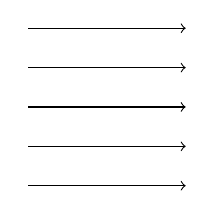
\begin{tikzpicture}
    \draw [->] (0,2) -- +(2,0);
    \draw [->] (0,1.5) -- +(2,0);
    \draw [->] (0,1) -- +(2,0);
    \draw [->] (0,0.5) -- +(2,0);
    \draw [->] (0,0) -- +(2,0);
  \end{tikzpicture}
  \caption{$t = 0$}
\end{subfigure}%
\begin{subfigure}{0.5\textwidth}
	\centering
	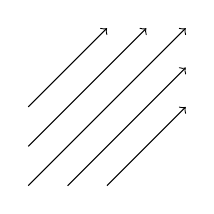
\begin{tikzpicture}
		\draw [->] (0,1) -- +(1,1);
		\draw [->] (0,0.5) -- +(1.5,1.5);
		\draw [->] (0,0) -- +(2,2);
		\draw [->] (0.5,0) -- +(1.5,1.5);
		\draw [->] (1,0) -- +(1,1);
	\end{tikzpicture}
	\caption{$t = 1$}
\end{subfigure}
\end{figure}

In contrast, a \emph{pathline}\index{pathline} is when we look at the trajectory of a fluid `particle' (which we can think of as a very small part of the fluid). The pathline $\mathbf{x} = \mathbf{x}(t; \mathbf{x}_0)$ of the particle that starts at $\mathbf{x}_0$ at $t = 0$ is found from
\[
\frac{\diff \mathbf{x}}{\diff t} = \mathbf{u}(\mathbf{x}, t)
,\]
with initial conditions $\mathbf{x} = \mathbf{x}_0$ at $t = 0$. The set of pathlines give the flow of one particle, at all times. The pathline of $\mathbf{u} = (1, t)$ is graphed in figure~\ref{fig:pathlines_1_t}.

\begin{figure}[h]
	\centering
	\caption{Pathlines of $\mathbf{u} = (1,t)$ for three initial points}
	\label{fig:pathlines_1_t}
	\begin{tikzpicture}
		\begin{axis}
			[
			xmin = 0,
			xmax = 3.1,
			ymin = 0,
			ymax = 1,
			axis lines = none
			]
		\addplot [domain = 0:1, smooth, ->] {x*x};
		\addplot [mark = *] coordinates {(0,0)};
		\addplot [domain = 1:2, smooth, ->] {(x-1) * (x-1)};
		\addplot [mark = *] coordinates {(1,0)};
		\addplot [domain = 2:3, smooth, ->] {(x-2) * (x-2)};
		\addplot [mark = *] coordinates {(2,0)};
	\end{axis}
	\end{tikzpicture}
\end{figure}

We can consider many particles, such as all $\mathbf{x}_0$ in a given region, to see how the shape and position of a dyed patch of fluid evolves. This is useful for thinking about transport and mixing problems.

For \emph{steady-state flows}\index{steady-state flows}, streamlines and pathlines are the same.

\subsection{The Material Derivative}
\label{sub:the_material_derivative}

Both streamlines and pathlines are taken from the Eulerian picture: we are sitting outside and watching the fluid go by. Things are different if we are drifting with the fluid.

In particular, for a field $F(\mathbf{x},t)$, which may be density or velocity or something else we want to know, we can measure it with respect to some fixed position. However, if we are moving along with the fluid, then this field is changing: we can parametrize it as $F(\mathbf{x}(t), t)$. We can calculate
\begin{align*}
	\delta F &= F(\mathbf{x} + \delta \mathbf{x}, t + \delta t) - F(\mathbf{x}, t) \\
		 &= \delta \mathbf{x} \cdot \nabla F + \delta t \frac{\partial F}{\partial t} + \mathcal{O}(\delta^2),
\end{align*}
and we know $\delta \mathbf{x} = \mathbf{u}(\mathbf{x},t) \delta t + \mathcal{O}(\delta^2)$, so these equations simplify to
\[
\frac{DF}{Dt} = \frac{\partial F}{\partial t} + \mathbf{u} \cdot \nabla F
,\]
where we use new notation for the total time derivative. The additional $\mathbf{u} \cdot \nabla F$ corresponds to the movement due to the fluid. This is called the \emph{material derivative}\index{material derivative}, as it describes the rate of change of a field, when moving through a fluid (or material).

\subsection{Conservation of Mass}
\label{sub:conservation_of_mass}

Consider a (rigid) tube with constant cross-section, with fluid coming in with speed $\mathbf{u} = 2$, and exiting with speed $\mathbf{u} = 1$.

For a fluid such as air, this could be conceivably possible: the air could be compressed in the tube.

However, with water this would be impossible, as the density of water $\rho_{\rm{water}}$ is relatively constant. Hence a difference in velocities means that mass is being destroyed.

This suggests that there must be a relationship between $\rho(\mathbf{x},t)$ and $\mathbf{u}(\mathbf{x},t)$ such that mass is never created or destroyed, so we go looking for such a relationship.

Consider an arbitrary volume $V$, fixed in space and bounded by a surface $\partial V$ with outwards normal $\mathbf{n}$. Then the mass in $V$, which is
\[
M = \int_{V} \rho \diff V
,\]
can only change if mass flows in or out at the surface $\partial V$. The amount of mass that escapes an area $A$ over time $t$ is $\rho \mathbf{u} \cdot \mathbf{n} \delta A \delta t$. We can think of $\rho \mathbf{u}$ as the \emph{mass flux}\index{mass flux}. Integrating over $V$,
\begin{align*}
	\frac{\diff}{\diff t} \int_{V} \rho \diff V &= - \int_{S} \rho \mathbf{u} \cdot \diff \mathbf{S}, \\
	\iff \int_{V} \frac{\partial p}{\partial t} \diff V &= - \int_{V} \nabla \cdot (\rho \mathbf{u}) \diff V,
\end{align*}
where we have used the divergence theorem. Since this holds for all volumes $V$, we must have
\[
\frac{\partial \rho}{\partial t} + \nabla \cdot (\rho \mathbf{u}) = 0
.\]
Using $\nabla \cdot (\rho \mathbf{u}) = \mathbf{u} \cdot \nabla \rho + \rho \nabla \cdot \mathbf{u}$, we can rewrite this as
\[
\frac{D \rho}{Dt} + \rho \nabla \cdot \mathbf{u} = 0
.\]
Physically, this means that if a fluid is flowing away from a point, the density should decrease, and vice versa.

If a fluid is \emph{incompressible}\index{incompressible}, then the density of the fluid is constant, so $\dot \rho = \nabla \rho = 0$. Hence the velocity must satisfy
\[
\nabla \cdot \mathbf{u} = 0
\]
for incompressible flow. In this course, we make the assumption that density is constant and uniform. This assumption is good when the speed of the fluid is much less than the speed of sound, which is around \qty{330}{\metre\per\second} in air, and \qty{1500}{\metre\per\second} in water.

\subsection{Kinematic Boundary Condition}
\label{sub:kinematic_boundary_condition}

Suppose that the material boundary of a body of fluid has velocity $\mathbf{U}(\mathbf{x},t)$. Then at a point $\mathbf{x}$ on the boundary of the fluid, the velocity relative to the moving boundary is $\mathbf{u}(\mathbf{x}, t) - \mathbf{U}(\mathbf{x}, t)$.

The condition that there is no mass flux across the boundary can be written as $\rho (\mathbf{u} - \mathbf{U}) \cdot \mathbf{n} \, \delta A \delta t=  0$, or
\[
\mathbf{n} \cdot \mathbf{u} = \mathbf{n} \cdot \mathbf{U}
.\]

\begin{exbox}
	\begin{enumerate}
		\item For a stationary rigid boundary, $\mathbf{U} = 0$, so we must have $\mathbf{u} \cdot \mathbf{n} = 0$.
		\item Water waves have an air-water interface $z = \eta(x, y, t)$. We can think of the water surface as a contour of the function $F(x, y, z, t) = z - \eta(x, y, t)$.

			Then the normal $\mathbf{n}$ will be parallel to $\nabla F = (-\eta_x, \eta_y, 1)$. Since $\mathbf{U} = (0, 0, \eta_t)$, if we take $\mathbf{u} = (u, v, w)$, the boundary flux condition implies
			\[
			- u \eta_x - v \eta_y + w = \eta_t
			.\]
			This is equivalent to
			\[
			\frac{D}{Dt}(z - \eta) = 0
			,\]
			which means that particles on the surface of the wave will stay on the surface.
	\end{enumerate}
\end{exbox}

\begin{figure}[h]
	\centering
	\caption{Surface of Water}
	\label{fig:water_surface}
	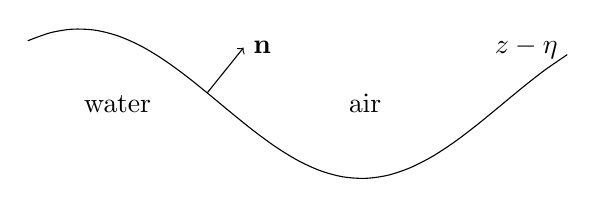
\begin{tikzpicture}
		\begin{axis}
			[
			xmin = 1,
			xmax = 7,
			ymin = -1,
			ymax = 1,
			axis lines = none
			]
			\addplot [smooth, domain = 1:7] {sin(deg(x))/3};
			\draw [->] (3,0.05) -- (3.4,0.25);
			\node [right] at (3.4, 0.25) {$\mathbf{n}$};
			\node at (4.75,0) {air};
			\node at (2,0) {water};
			\node [left] at (7, 0.25) {$z - \eta$};
		\end{axis}
	\end{tikzpicture}
\end{figure}

\subsection{Stream Function for 2D Incompressible Flow}
\label{sub:stream_function_for_2d_incompressible_flow}

Recall that a fluid is incompressible if $\nabla \cdot \mathbf{u} = 0$. However, this is equivalent to $\mathbf{u} = \nabla \times \mathbf{A}$ for some potential $\mathbf{A}$.

For two dimensional flows $\mathbf{u} = (u(x,y),v(x,y),0)$, we can take
\[
\mathbf{A} = (0, 0, \psi(x, y)) \implies \mathbf{u} = \biggl( \frac{\partial \psi}{\partial y}, - \frac{\partial \psi}{\partial x}, 0 \biggr)
.\]
Indeed, this implies
\[
\frac{\partial u}{\partial x} + \frac{\partial v}{\partial y} = 0
,\] 
so $\mathbf{u}$ is divergence-free, as expected. We say that $\psi(x, y)$ is the \emph{stream function}\index{stream function}.

The stream function satisfies the following properties:
\begin{enumerate}[(i)]
	\item The streamlines are given by $\psi = C$ (so $\mathbf{u}$ is parallel to the contours of $\psi$).
	\item $|\mathbf{u}| = |\nabla \psi|$, so the flow is faster where the streamlines are closer together.
	\item The volume that is crossing the line from $\mathbf{x}_0$ to $\mathbf{x}_1$ is
		\[
		\int_{\mathbf{x}_0}^{\mathbf{x}_1} \mathbf{u} \cdot \mathbf{n} \diff l = \psi(\mathbf{x}_1) - \psi(\mathbf{x}_0)
		.\]
	\item $\psi$ is constant on a stationary rigid boundary.
\end{enumerate}

\begin{exbox}
	Take $\mathbf{u} = (y, x)$. Since $\nabla \cdot \mathbf{u} = 0$, a stream function exists. Integrating the above equations,
	\begin{align*}
		\frac{\partial \phi}{\partial y} = y &\implies \psi = \frac{1}{2} y^2 + f(x), \\
		-\frac{\partial \psi}{\partial x} = x &\implies f(x) = -\frac{1}{2}x^2.
	\end{align*}
	Hence the streamlines are
	\[
		y^2 - x^2 = C
	.\]
\end{exbox}

In polar coordinates, we have $\mathbf{u} = (u_r(r, \theta), u_\theta(r, \theta), 0)$. If $\mathbf{A} = (0, 0, \psi(r, \theta))$, then
\[
\mathbf{u} = \nabla \times \mathbf{A} = \biggl( \frac{1}{r} \frac{\partial \psi}{\partial \theta}, - \frac{\partial \psi}{\partial r}, 0 \biggr)
.\]
We can verify that
\[
\nabla \cdot \mathbf{u} = \frac{1}{r} \frac{\partial}{\partial r} (r u_r) + \frac{1}{r} \frac{\partial u_{\theta}}{\partial \theta} = 0
.\]

Axisymmetric flow in spherical polar coordinates has
\[
u_{\phi} = \frac{\partial}{\partial \phi} = 0
.\]
If we have $\nabla \cdot \mathbf{u} = 0$, and we take
\[
\mathbf{A} = \biggl( 0, 0, \frac{\Psi(r, \theta)}{r \sin \theta} \biggr)
,\]
then
\[
\mathbf{u} = \biggl( \frac{1}{r^2 \sin \theta} \frac{\partial \Psi}{\partial \theta}, - \frac{1}{r \sin \theta} \frac{\partial \Psi}{\partial r}, 0 \biggr)
\]
is parallel to the contours of $\Psi$. Hence the contours of the Stokes stream $\Psi(r, \theta)$ form the stream tubes.

\newpage

\section{Dynamics of Inviscid Flow}
\label{sec:dynamics_of_inviscid_flow}

\subsection{Surface and Volume Forces}
\label{sub:surface_and_volume_forces}

There are two types of force which act on a fluid:
\begin{enumerate}[(i)]
	\item Those proportional to the volume, like gravity.
	\item Those proportional to the surface area, like pressure or \emph{viscous stress}, which is the friction between moving fluid and moving material, whether a boundary or another fluid.
\end{enumerate}
We look at these individually.

\begin{enumerate}[(i)]
	\item For \emph{volume} or \emph{body forces}\index{volume force}\index{body force}, we denote the force on a small volume element as $\mathbf{f}(\mathbf{x},t)\, \delta V$. Often, $\mathbf{f}$ is \emph{conservative}with potential energy per unit volume $\chi$, and hence $\mathbf{f} = - \nabla \chi$.

		The most common case for us is gravity; here $\mathbf{f} \, \delta V = \rho \mathbf{g} \, \delta V$, with $\chi = \rho g z$, where $\mathbf{g} = (0, 0, g)$.
	\item For a \emph{surface force}\index{surface force}, we consider a small element of area $\mathbf{n} \, \delta A$.

		Denote the surface force exerted by the outside on the inside by $\bm{\tau}(\mathbf{x}, t ; \mathbf{n}) \, \delta A$, where $\bm{\tau}$ is the \emph{stress}\index{stress} acting on the area element. Note that the stress $\bm{\tau}$ depends on the orientation $\mathbf{n}$.

		By Newton's third law, the surface force exerted by the inside on the outside is
		\[
		- \bm{\tau}(\mathbf{x}, t;\mathbf{n}) = \bm{\tau}(\mathbf{x}, t; \mathbf{n})
		.\]
		We defer discussion of viscous stresses to chapter 3. In fact, in many phenomena the viscous stresses are negligible and the fluid behaves as if it is \emph{inviscid}\index{inviscid} (frictionless).
\end{enumerate}


\begin{figure}[h]
	\centering
	\caption{Surface force on a small area $\delta A$}
	\label{fig:surface_force}
	\begin{tikzpicture}
		\draw (0,0) circle [x radius = 1,y radius = 2];
		\draw [->, thick] (0,0) -- +(2,0);
		\draw [->, thick, red] (-1,0) -- +(-1.5,0);
		\node at (-2,-1) {$\bm{\tau} = - p \mathbf{n}$};
		\node at (3, 1) {outside};
		\node at (-3, 1) {inside};
		\node [right] at (2,0) {$\mathbf{n}\, \delta A$};
	\end{tikzpicture}
\end{figure}

For inviscid fluids, the stress $\bm{\tau}$ acting across $\mathbf{n} \, \delta A$ has no tangential component, and has magnitude independent of the orientation:
\[
\bm{\tau}(\mathbf{x},t;\mathbf{n}) = - p(\mathbf{x},t)\mathbf{n}
,\]
where $p$ is the pressure. Note the sign: the outside pushes on the inside in the direction $- \mathbf{n}$.

\subsection{The Euler Momentum Equation}
\label{sub:the_euler_momentum_equation}

Consider an arbitrary volume $V$, fixed in space, bounded by surface $\partial V$ with an outward normal $\mathbf{n}$.

The momentum $\int_{V} p \mathbf{u}\diff V$ inside $V$ can change due to:
\begin{enumerate}[(i)]
	\item Flow of momentum across the boundary $\partial V$,
	\item Volume/body forces,
	\item Surface Forces.
\end{enumerate}

Recall the volume out across $\delta A$ in time $\delta t$ is $\mathbf{n} \, \delta A \cdot \mathbf{u} \, \delta t$, and the momentum out is $\rho \mathbf{u} (\mathbf{u} \cdot \mathbf{n} \, \delta A \delta t)$. Hence,
\[
\frac{\diff}{\diff t} \int_{V} \rho \mathbf{u} \diff V = - \int_{\partial V} \rho \mathbf{u}(\mathbf{u} \cdot \mathbf{n}) \diff A + \int_{\partial V} (- p \mathbf{n}) \diff A + \int_{V} \mathbf{f} \diff V
.\]

Here $\rho u_i u_j$ is the momentum flux, a second order tensor. We can rewrite this in terms of components as
\begin{align*}
	\frac{\diff}{\diff t} \int_{V} \rho u_i \diff V &= - \int_{\partial V} (\rho u_i u_j) n_j \diff A - \int_{\partial V} p n_i \diff A + \int_{V} f_i \diff V \\
	\iff \int_{V} \frac{\partial}{\partial t} (\rho u_i) \diff V &= - \int_{V} \frac{\partial}{\partial x_j} (\rho u_i u_j) \diff V - \int_{V} \frac{\partial f}{\partial x_i} \diff V + \int_{V} f_i \diff V.
\end{align*}
Since $V$ is arbitrary, we obtain
\[
\frac{\partial}{\partial t}(\rho u_i) + \frac{\partial}{\partial x_j}(\rho u_i u_h) = - \frac{\partial f}{\partial x_i} + f_i
.\]
The left hand side can be expanded as
\begin{align*}
	LHS &= u_i \biggl( \frac{\partial \rho}{\partial t} + \frac{\partial}{\partial x_j} (\rho u_j)\biggr) + \rho \frac{\partial u_i}{\partial t} + \rho u_j \frac{\partial u_i}{\partial x_j} \\
	    &= \rho \biggl(\frac{\partial}{\partial t} + \mathbf{u} \cdot \nabla\biggr) u_i,
\end{align*}
due to mass conservation. What we are left with is the material derivative, so we get
\[
\rho \frac{D \mathbf{u}}{D t} = - \nabla p + \mathbf{f}
.\]
This is the \emph{Euler momentum equation}\index{Euler momentum equation}.

The Euler momentum equation also has a dynamic boundary condition, which says that the stress $\bm{\tau}$ exerted on the fluid by the boundary is $-p \mathbf{n}$.

\begin{exbox}
	Consider a bent hose pipe with steady uniform flow $U$ in and out, with constant cross-sectional area $A$. We neglect gravity (so $\mathbf{f} = 0$).

	From the momentum integral equation, the momentum inside the volume is unchanging, and $\mathbf{f} = 0$, so this simplifies to
	\[
		\int_{\rm{walls}} [\rho \mathbf{u}(\mathbf{u} \cdot \mathbf{n}) + p \mathbf{n}] \diff A + \int_{\rm{ends}} [\rho \mathbf{u} (\mathbf{u} \cdot \mathbf{n}) + p \mathbf{n}] \diff A = 0
	.\]
	We know that
	\[
		\int_{\rm{walls}} [\rho \mathbf{u}(\mathbf{u} \cdot \mathbf{n}) + p \mathbf{n}] \diff A = \int_{\rm{walls}} p \mathbf{n} \diff A
	,\]
	as the walls are rigid, so $\mathbf{u} \cdot \mathbf{n} = 0$. This is simply the force by the fluid on the pipe. Moreover, on the ends
	\[
		\int_{\rm{ends}}[\rho \mathbf{u}(\mathbf{u} \cdot \mathbf{n}) + p \mathbf{n}] \diff A = A [p_1 \mathbf{n}_1 + \rho(-U \mathbf{n}_1)(-U) + p_2 \mathbf{n}_2 + \rho(U \mathbf{n}_2)U]
	.\]
	In fact we get $p_1 = p_2$. Hence the force on the pipe is
	\[
	-A (p + \rho U^2)(\mathbf{n}_1 + \mathbf{n}_2)
	.\]
	The $\rho U^2$ contribution comes from the change in momentum flux: the fluid in changes direction.
\end{exbox}


\newpage

\printindex

\end{document}
